\documentclass[
	% -- opções da classe memoir --
	12pt,				% tamanho da fonte
	openright,			% capítulos começam em pág ímpar (insere página vazia caso preciso)
	oneside,			% para impressão em frente e verso. Oposto a oneside
	a4paper,			% tamanho do papel.
	% -- opções da classe abntex2 --
	chapter=TITLE,		% títulos de capítulos convertidos em letras maiúsculas
	%section=TITLE,		% títulos de seções convertidos em letras maiúsculas
	%subsection=TITLE,	% títulos de subseções convertidos em letras maiúsculas
	%subsection=TITLE,% títulos de subseções convertidos em letras maiúsculas
	% -- opções do pacote babel --
	english,			% idioma adicional para hifenização
	french,				% idioma adicional para hifenização
	spanish,			% idioma adicional para hifenização
	brazil				% o último idioma é o principal do documento
	]{abntex2}
% ---
% Pacotes básicos 
% ---
\usepackage{lmodern}			% Usa a fonte Latin Modern
\usepackage{mathptmx}			% Usa a fonte Times New Roman
\usepackage[T1]{fontenc}		% Selecao de codigos de fonte.
\usepackage[utf8]{inputenc}		% Codificacao do documento (conversão automática dos acentos)
\usepackage{lastpage}			% Usado pela Ficha catalográfica
\usepackage{indentfirst}		% Indenta o primeiro parágrafo de cada seção.
\usepackage{color}				% Controle das cores
\usepackage{graphicx}			% Inclusão de gráficos
\usepackage{subcaption}				% Inclusão de gráficos lado a lado
\usepackage{microtype} 			% para melhorias de justificação
\usepackage{tabularx,ragged2e}	% Para inserir tabelas
\usepackage{multirow}			% Para mesclar células\documentclass[
\usepackage[dvipsnames,table,xcdraw]{xcolor}		% Permite adicionar cores nas linhas de tabelas
\usepackage{fancyvrb}			% Permite adicionar arquivos de texto
\usepackage[portuguese, ruled, linesnumbered]{algorithm2e} % Uso de algoritmos
\usepackage{amsfonts}			% Permite usar notação de conjuntos
\usepackage{amsmath}			% Permite citar equações
\usepackage{amsthm}				% Permite criar teoremas e experimentos
\usepackage[font={bf, small}, labelsep=endash, labelfont=bf]{caption}	% Faz legenda de figuras ficarem em negrito
\usepackage{cancel}				% Permite fazer expressão tendendo a zero
\usepackage{epstopdf}			% Converte eps para pdf
\usepackage[final]{pdfpages}
\usepackage{hyperref}
\usepackage{fancybox}
\usepackage{float}

\usepackage{listings} % Para incluir código Python
\usepackage{geometry} % Para ajustar as margens
\usepackage{xcolor}


\geometry{margin=1in}

\newcolumntype{L}{>{\RaggedRight\arraybackslash}X}
% ---
% ---
% Pacotes adicionais, usados apenas no âmbito do Modelo Canônico do abnteX2
% ---
\usepackage{lipsum}				% para geração de dummy text
% ---
% ---
% Pacotes de citações
% ---
%\usepackage[brazilian,hyperpageref]{backref}	 % Paginas com as citações na bibl
\usepackage[alf, abnt-emphasize=bf]{abntex2cite}	% Citações padrão ABNT
% ---
% Customizações para o layout da UFPA
% ---
\usepackage{modelo-ufpa/ufpa}
% Muda o título de lista de ilustrações para lista de figuras
\addto\captionsbrazil{%
  \renewcommand{\listfigurename}%
    {Lista de Ilustrações}%
	\renewcommand{\listtablename}%
    {Lista de Tabelas}%
}
% Permite utilizar figuras sem precisar colocar o caminho absoluto
\graphicspath{{imagens/}}
% Define o ambiente de experimentos
\theoremstyle{definition}
\newtheorem{experimento}{Experimento}[section]
\newcommand{\experimentoautorefname}{Experimento}


% --------------------------------------------------------------
% Informações do TRABALHO
% --------------------------------------------------------------
\universidade{UNIVERSIDADE FEDERAL DO PARÁ}
\instituto{INSTITUTO DE TECNOLOGIA}
\faculdade{FACULDADE DE COMPUTAÇÃO E TELECOMUNICAÇÕES}
%\curso{CURSO DE BACHARELADO EM SISTEMAS DE INFORMAÇÃO}
\titulo{RELATÓRIO DE SISTEMAS OPERACIONAIS}
\autor{
%\begin{tabular}{l l}
    DAVID PINHEIRO DE SOUSA - 202207040045 \\
    JOAO VICTOR SANTOS BRITO FERREIRA - 202207040028 \\
    JOEL TAVARES MIRANDA - 202206840054 \\
    KAUAN MIRANDA TAVARES - 202206840033 \\
    MARCO ANTONIO DO ESPIRITO SANTO MAUES JUNIOR - 202206840038 \\
%\end{tabular}
}
\local{Belém}
\data{2023}
\orientador{Prof. Dr. Diego Lisboa Cardoso}
\tipotrabalho{Monografia}

% o nome da instituição e a área de concentração 
\preambulo{Relatório do trabalho 6 de Sistemas Operacionais.}
%\sobrenome{Sobrenome}
%\nome{Nome}
%\palavraschave
%\datadadefesa{Data da Defesa: 09 de Março de 2017}%07 de Dezembro de 2016}
\conceito{Conceito: Excelente}
\faculdadedoorientador{Faculdade de Biotecnologia - UFPA}
\primeiromembrodabanca{Prof. Dr. Nome Sobrenome}
\faculdadedoprimeiromembrodabanca{Faculdade de Computação - UFPA}
\segundomembrodabanca{Prof. Dra. Nome Sobrenome}
\faculdadedosegundomembrodabanca{Faculdade de Biotecnologia - UFPA}
% -------------------------------------------------------------------------
% ---
% Configurações de aparência do PDF final
% alterando o aspecto da cor azul
\definecolor{blue}{RGB}{41,5,195}
% informações do PDF
\makeatletter
\hypersetup{
     	%pagebackref=true,
		pdftitle={\imprimirtitulo}, 
		pdfauthor={\imprimirautor},
    	pdfsubject={\imprimirpreambulo},
	    pdfcreator={LaTeX with abnTeX2},
		pdfkeywords={\imprimirpalavraschave}, 
		colorlinks=true,       		% false: boxed links; true: colored links
    	linkcolor=black,          	% color of internal links
    	citecolor=black,        		% color of links to bibliography
    	filecolor=magenta,      		% color of file links
		urlcolor=blue,
		bookmarksdepth=4,
        breaklinks=true
}
\makeatother
% --- 
% Espaçamentos entre linhas e parágrafos 
% --- 
% O tamanho do parágrafo é dado por:
\setlength{\parindent}{1.3cm}
% Controle do espaçamento entre um parágrafo e outro:
\setlength{\parskip}{0.2cm}  % tente também \onelineskip
% compila o indice
% ---
\makeindex
% ---

% -------------------------------------------------------------------------
% ---------------------------INICIO DO DOCUMENTO---------------------------
% -------------------------------------------------------------------------
\begin{document}
% Seleciona o idioma do documento (conforme pacotes do babel)
\selectlanguage{brazil}
% Retira espaço extra obsoleto entre as frases.
\frenchspacing 
% ----------------------------------------------------------
% ELEMENTOS PRÉ-TEXTUAIS
% ----------------------------------------------------------
% \pretextual

% ---
% Capa
% ---
\imprimircapa
% ---

% ---
% Folha de rosto

\imprimirfolhaderosto

\newpage

\setlength{\absparsep}{18pt} % ajusta o espaçamento dos parágrafos do resumo

\pdfbookmark[0]{\contentsname}{toc}
\tableofcontents*
\cleardoublepage
% ---
% ---------------------------------------------------------
% ELEMENTOS TEXTUAIS
% ----------------------------------------------------------
\textual

% ----------------------------------------------------------
% Introdução
% ----------------------------------------------------------

\chapter{Introdução}
O sistema de arquivos é uma peça fundamental para o gerenciamento eficiente de dados em 
sistemas operacionais. Entre as diversas opções disponíveis, a escolhida para este trabalho 
foi o sistema de arquivos ext4, ou Quarta Extensão, que destaca-se como uma escolha proeminente para ambientes 
baseados em Linux. Ao longo deste trabalho serão apresentados diversos aspectos, características e benchmarks de desempenho 
do sistema ext4.

\chapter{Apresentação do Sistema}
O Ext4, abreviação de Fourth Extended Filesystem, surge como uma evolução do sistema de arquivos Ext3, sendo desenvolvido especificamente para atender às crescentes demandas do sistema operacional Linux. A concepção do Ext4 foi motivada pela necessidade de superar as limitações do Ext3, adaptando-se às exigências modernas no tratamento e processamento de dados.

Com o propósito de estabelecer um ambiente de armazenamento mais eficiente e confiável, o Ext4 introduz avanços notáveis em capacidade, desempenho e segurança. Sua arquitetura foi cuidadosamente planejada para suportar volumes de dados consideravelmente maiores, proporcionando maior flexibilidade para enfrentar as demandas crescentes das aplicações contemporâneas.

A notável capacidade do sistema de arquivos Ext4, com um tamanho máximo teórico de 1 exabyte, o posiciona como uma escolha ideal para lidar com grandes volumes de dados em ambientes Linux, oferecendo suporte a sistemas de arquivos consideravelmente amplos.

Quanto à velocidade, o Ext4 destaca-se por melhorias significativas em comparação com o Ext3, principalmente devido à implementação de extensões. Ao organizar os dados em blocos contíguos, o Ext4 reduz a fragmentação, aprimorando a eficiência no acesso aos dados e otimizando o desempenho global do sistema.

A expansão do tamanho máximo do arquivo para 16 terabytes proporciona uma flexibilidade substancial ao lidar com arquivos grandes. Essa ampliação é crucial em ambientes que demandam o armazenamento e a manipulação de dados massivos, assegurando que o Ext4 atenda plenamente às exigências de cenários envolvendo arquivos consideravelmente grandes. Assim, o Ext4 se destaca como uma solução coesa e abrangente para os desafios contemporâneos de armazenamento no universo Linux.

\chapter{Sistema de Alocação de Arquivos}
%Explicação sobre como o ext4 aloca arquivos no disco.
No Ext4 o a alocação de arquivos desempenha um papel vital na organização e na gestão eficiente do espaço em disco. 
Dito isso, o Ext4 utiliza uma estrutura aprimorada em comparação aos seus predecessores, Ext2 e Ext3, para otimizar o 
o desempenho e a eficiência, a seguir são apresentados alguns aspectos da alocação no Ext4

%\section{Extensões (Extents)}
%Uma das melhorias significativas introduzidas no Ext4 é o conceito de \textit{extensões} ou \textit{extents}. Em vez de manter listas detalhadas de blocos individuais para armazenar dados de um arquivo, o Ext4 organiza os dados em extensões, que são sequências de blocos contíguos. Essa abordagem ajuda a reduzir a fragmentação do sistema de arquivos, melhorando a eficiência no acesso aos dados.

\section{Alocação por Bloco Indireto}
A alocação por bloco indireto é uma técnica avançada utilizada no sistema de arquivos \texttt{ext}, 
proporcionando uma gestão eficiente de grandes quantidades de dados. Essa estratégia utiliza uma 
estrutura adicional, chamada bloco indireto, para otimizar o acesso e a alocação de dados.

Ao lidar com arquivos extensos, a alocação por bloco indireto permite a criação de uma camada 
adicional entre os blocos de dados e o inode. Em vez de armazenar diretamente os endereços dos 
blocos de dados no inode, é utilizado um bloco indireto. Esse bloco indireto contém endereços 
de blocos de dados, proporcionando uma abstração eficiente para acessar grandes volumes de dados.

\subsection{Vantagens}
A alocação por bloco indireto apresenta diversas vantagens:

\begin{itemize}
    \item \textbf{Gestão Eficiente de Grandes Arquivos:} Permite a manipulação eficiente de arquivos grandes, facilitando a alocação dinâmica de blocos de dados.
    
    \item \textbf{Redução de Overhead no Inode:} Ao utilizar blocos indiretos, o inode permanece compacto, reduzindo o overhead associado a armazenar uma grande quantidade de endereços de bloco diretamente.
    
    \item \textbf{Acesso Rápido:} Simplifica o acesso a grandes conjuntos de dados, promovendo um acesso mais rápido e eficiente.
\end{itemize}

\subsection{Implementação Prática}
A implementação prática da alocação por bloco indireto no sistema de arquivos \texttt{ext} envolve a criação de um bloco indireto durante a criação do arquivo. Por exemplo:

\begin{lstlisting}[language=bash, caption={Exemplo de Alocação por Bloco Indireto}]
$ touch arquivo_grande.txt  
$ chattr +i bloco_indireto.txt  
$ chattr +B bloco_indireto.txt arquivo\_grande.txt  
\end{lstlisting}

Neste exemplo, um bloco indireto é criado e associado ao arquivo \texttt{arquivo\_grande.txt} para otimizar a alocação de blocos de dados.

A alocação por bloco indireto é uma estratégia avançada que contribui para a eficiência e desempenho do sistema de arquivos \texttt{ext}, especialmente ao lidar com grandes volumes de dados.

\section{Tamanho de Bloco Variável}
A abordagem de tamanho de bloco variável é uma característica avançada do sistema de arquivos \texttt{ext}, permitindo a flexibilidade na alocação de espaço em disco, especialmente ao lidar com diferentes tipos de arquivos.

Ao contrário de sistemas de arquivos com tamanho de bloco fixo, o \texttt{ext} oferece a capacidade de variar o tamanho dos blocos de dados. Cada arquivo pode ser associado a um tamanho de bloco específico, ajustando-se dinamicamente às necessidades do conteúdo. Isso significa que arquivos pequenos podem compartilhar blocos com outros, enquanto arquivos maiores podem ter blocos maiores, otimizando a utilização do espaço em disco.

\subsection{Vantagens}
A implementação de tamanho de bloco variável apresenta várias vantagens:

\begin{itemize}
    \item \textbf{Otimização de Espaço:} Permite uma alocação mais eficiente de espaço, especialmente para arquivos de diferentes tamanhos.
    
    \item \textbf{Redução de Fragmentação:} Ao adaptar o tamanho do bloco às necessidades do arquivo, a fragmentação é reduzida, contribuindo para um melhor desempenho do sistema.
    
    \item \textbf{Flexibilidade para Diferentes Tipos de Arquivos:} A capacidade de escolher tamanhos de bloco específicos para diferentes tipos de arquivos otimiza o desempenho e a gestão de recursos.
\end{itemize}

\subsection{Implementação Prática}
A implementação prática do tamanho de bloco variável no sistema de arquivos \texttt{ext} envolve a configuração do tamanho de bloco no momento da formatação do sistema de arquivos. Por exemplo:

\begin{lstlisting}[language=bash, caption={Exemplo de Tamanho de Bloco Variável}]
$ mkfs.ext4 -b 4096 -O ^uninit_bg /dev/sdX1
\end{lstlisting}

Neste exemplo, o comando \texttt{mkfs.ext4} é utilizado para formatar a partição \texttt{/dev/sdX1} com um tamanho de bloco de 4096 bytes.

A capacidade de ajustar dinamicamente o tamanho do bloco oferece uma abordagem flexível e eficiente na gestão do espaço em disco no sistema de arquivos \texttt{ext}.

\section{Alocação Pré-Alocada no Sistema de Arquivos \texttt{ext}}
A alocação pré-alocada é uma técnica no sistema de arquivos \texttt{ext} que envolve a reserva antecipada de espaço em disco para um arquivo, mas com uma abordagem mais flexível em comparação com a alocação por reservas convencional.

Ao contrário da alocação por reservas, onde um tamanho fixo é reservado antecipadamente, a alocação pré-alocada permite que um arquivo solicite uma quantidade inicial de espaço e, ao longo do tempo, solicite mais espaço conforme necessário. Isso proporciona uma flexibilidade dinâmica, permitindo a adaptação do tamanho do arquivo sem a necessidade de uma reserva estática.

\subsection{Vantagens}
A alocação pré-alocada oferece diversas vantagens:

\begin{itemize}
    \item \textbf{Flexibilidade Dinâmica:} Os arquivos podem crescer dinamicamente, solicitando mais espaço à medida que necessário, evitando reservas estáticas excessivas.
    
    \item \textbf{Otimização do Uso de Espaço:} O sistema pode otimizar o uso de espaço em disco, alocando eficientemente apenas a quantidade necessária.
    
    \item \textbf{Manutenção de Desempenho:} Evita a fragmentação excessiva, mantendo um desempenho consistente ao longo do tempo.
\end{itemize}

\subsection{Implementação Prática}
A implementação prática da alocação pré-alocada no sistema de arquivos \texttt{ext} envolve o uso de comandos específicos durante a criação ou manipulação de arquivos. Por exemplo:

\begin{lstlisting}[language=bash, caption={Exemplo de Alocação Pré-Alocada}]
$ fallocate -l 1G arquivo_prealocado.txt  
$ echo "Novo conteudo" >> arquivo_prealocado.txt   
\end{lstlisting}

Neste exemplo, o comando \texttt{fallocate} é utilizado para alocar inicialmente 1 gigabyte para o arquivo \texttt{arquivo\_prealocado.txt}. Conforme o conteúdo é adicionado, o sistema pode alocar mais espaço conforme necessário.

A alocação pré-alocada oferece uma abordagem dinâmica para o gerenciamento de espaço em disco, adaptando-se às necessidades variáveis dos arquivos ao longo do tempo.

\chapter{Gestão do Espaço Livre no Ext4}

A eficiente gestão do espaço livre é uma componente crucial para garantir o desempenho, a confiabilidade e a 
integridade do sistema de arquivos Ext4. Neste capítulo, exploraremos algumas estratégias e características 
fundamentais implementadas no Ext4 para otimizar o uso do espaço disponível e minimizar a fragmentação.

\section{Bitmap de Blocos Livres}

O Bitmap de Blocos Livres é uma estrutura essencial no sistema de arquivos \texttt{ext}, desempenhando um papel crucial na gestão e alocação de espaço em disco. Este mecanismo utiliza um mapa de bits para representar o estado de cada bloco no disco, indicando se um bloco está ocupado ou livre.

Cada bloco de dados no sistema de arquivos \texttt{ext} é associado a um bit no Bitmap de Blocos Livres. Se o bit correspondente estiver definido como "livre", o bloco está disponível para alocação. Caso contrário, se o bit estiver definido como "ocupado", o bloco já está sendo utilizado por algum arquivo.

\subsection{Vantagens}
O uso do Bitmap de Blocos Livres oferece diversas vantagens significativas:

\begin{itemize}
    \item \textbf{Eficiência na Alocação:} O mapa de bits permite uma verificação rápida e eficiente da disponibilidade de blocos, facilitando a alocação de espaço para novos arquivos.
    
    \item \textbf{Desempenho Aprimorado:} A rápida identificação de blocos livres contribui para um melhor desempenho do sistema durante as operações de leitura e gravação.
    
    \item \textbf{Simplicidade na Gestão:} A estrutura simplificada do Bitmap de Blocos Livres facilita a implementação e a manutenção do sistema de arquivos.
\end{itemize}

\subsection{Implementação Prática}
A manipulação do Bitmap de Blocos Livres pode ser realizada por meio de comandos específicos no sistema de arquivos \texttt{ext}. Por exemplo:

\begin{lstlisting}[language=bash, caption={Exemplo de Manipulação do Bitmap de Blocos Livres}]
$ dumpe2fs /dev/sda1 | grep "Free blocks"
\end{lstlisting}

Este comando exibe informações sobre os blocos livres no sistema de arquivos montado em \texttt{/dev/sda1}.

\section{Trim/Discard}

O comando \texttt{trim} (ou \texttt{discard}) é uma operação essencial em sistemas de arquivos modernos, projetada para melhorar a eficiência do gerenciamento de espaço em dispositivos de armazenamento de estado sólido (SSD). Esta operação permite que o sistema operacional notifique o dispositivo de armazenamento sobre blocos de dados que não estão mais em uso, permitindo a liberação física desses blocos.

Quando dados são excluídos de um sistema de arquivos em dispositivos SSD, os blocos correspondentes podem não ser imediatamente liberados. O comando \texttt{trim} atua informando ao dispositivo de armazenamento que determinados blocos não estão mais em uso e podem ser apagados. Isso resulta em uma melhor gestão do espaço livre e ajuda a manter o desempenho de gravação em níveis ótimos.

\subsection{Vantagens}
A utilização do comando \texttt{trim}/\texttt{discard} oferece várias vantagens:

\begin{itemize}
    \item \textbf{Melhor Desempenho:} Ao liberar blocos não utilizados, evita-se a sobrecarga de gravação e mantém-se o desempenho do SSD.
    
    \item \textbf{Aumento da Vida Útil do SSD:} Reduz o desgaste do SSD, uma vez que a operação de descarte evita regravações desnecessárias.
    
    \item \textbf{Otimização do Espaço:} Libera espaço não utilizado, aumentando a eficiência global do sistema de armazenamento.
\end{itemize}

\subsection{Implementação Prática}
Em sistemas de arquivos que suportam a operação de descarte, como o \texttt{ext4}, o comando \texttt{fstrim} pode ser utilizado para enviar a instrução de descarte manualmente. Exemplo:

\begin{lstlisting}[language=bash, caption={Exemplo de Utilização do \texttt{fstrim}}]
$ sudo fstrim /
\end{lstlisting}

Este comando enviará uma instrução de descarte para o sistema de arquivos na partição raiz.

%%%%%%%%%%%%%%%%%%%%%%%%%%%%%%%%%%%%%%%%%%%%%%%%%%%%%%%%%%%%%%%%%%%%%%%%%%%%%%%%%%%%%%%%%%%%5

\chapter{Estrutura do Sistema de Arquivos}
%Descrição da estrutura interna do ext4, destacando a organização em grupos de blocos.

A estruturta do Ext4 é bastante semelhante a de seus antecessores, com a adição de novos campos para 
suportar números de bloco de 64 bits. Até o momento, os campos de carimbo de data e hora no superbloco 
ainda são de 32 bits e não possuem um campo de bits mais significativos associado a eles; no entanto, 
destaca-se que o campo \texttt{s\_log\_groups\_per\_flex} desempenha um papel crucial na organização 
dos grupos de blocos. Nas versões mais recentes do kernel, o superbloco também incorpora campos 
destinados ao rastreamento de erros e à criação de snapshots.

%%%%%%%%%%%%%%%%%%%%%%%%%%%%%

\section{Journaling}\label{sec:journaling}

O \textit{journaling} é uma técnica utilizada por sistemas de arquivos em situações de 
recuperação de falhas. Ele oferece um tempo reduzido de recuperação em troca de sobrecarga 
adicional no sistema de arquivos em termos de tempo e/ou espaço. O \textit{journal}, 
assume a forma de um registro de tamanho fixo que regularmente se sobrescreve. Ações são 
registradas no \textit{journal} e reproduzidas na íntegra ou não durante a recuperação do 
sistema de arquivos. Essa característica, chamada de atomicidade, permite que o Ext4 alcance 
um estado consistente mais rapidamente do que por meio de um programa de verificação de sistema 
de arquivos, como o \texttt{e2fsck}.

A ação real de \textit{journaling} é tratada separadamente do sistema de arquivos 
pelo \textit{Journal Block Device}. O sistema de arquivos Ext é usado para identificar 
transações que são então repassadas ao \textit{Journal Block Device} para serem registradas. 
Uma transação é um conjunto de atualizações enviadas ao dispositivo e identificadas unicamente 
por números de sequência. O número de sequência da transação é utilizado em blocos de descritor 
e de confirmação para denotar o início e o fim de uma transação, respectivamente. Os dados que 
estão sendo registrados no \textit{journal} estão entre os blocos de descritor e de confirmação. 
O bloco de descritor também contém uma lista dos blocos do sistema de arquivos que são atualizados 
durante uma transação. É importante observar que o bloco de confirmação só é criado depois 
que os dados do sistema de arquivos foram registrados no disco para garantir a atomicidade.

Existe também um bloco de revogação. Este, assim como o bloco de descritor, possui um 
número de sequência e uma lista de blocos do sistema de arquivos, mas seu propósito é 
evitar alterações durante o processo de recuperação. Qualquer bloco do sistema de arquivos 
listado no bloco de revogação que também está em uma transação não confirmada com um número 
de sequência inferior ao do bloco de revogação não será restaurado.

A próxima estrutura que o \textit{journal} utiliza é provavelmente uma das mais 
importantes: o \textit{superblock}. Isso não deve ser confundido com o 
\textit{superblock} do sistema de arquivos, pois é específico para o \textit{journal}. 
Esta estrutura tem a tarefa de identificar o primeiro bloco de descritor no \textit{journal}. 
O uso do \textit{journal} como um registro circular torna essa tarefa necessária, já 
que não pode ser assumido que o início do \textit{journal} está localizado no início de 
seu espaço de armazenamento físico \cite{carrier2005file}. A relação entre os diferentes 
tipos de blocos de \textit{journal} é exibida na Figura \ref{fig:ext3_joual_blocks}. Nesta figura, a transação 55 
está completa, pois o conjunto de blocos de metadados associados a ela está incluído em 
um bloco de descritor e bloco de confirmação. No entanto, a transação 56 não foi concluída, 
então nenhum bloco de confirmação foi criado. Quando o sistema de arquivos é montado 
novamente e o \textit{journal} verificado, um bloco de revogação será criado. Como a 
transação 56 não possui um bloco de confirmação e possui um número de sequência inferior 
a 57, as alterações associadas a esta transação não serão reproduzidas.

\begin{figure}[h]
    \centering
    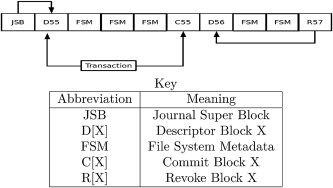
\includegraphics[width=0.5\textwidth]{journalingf.jpg}
    \caption{Blocos de \textit{journal} do Ext3. Adaptado de \cite{carrier2005file}.}
    \label{fig:ext3_joual_blocks}
\end{figure}

Os três modos documentados de \textit{journaling} são \textit{Journal}, \textit{Ordered} e 
\textit{Writeback} \cite{bovet_cesati_2005}. O modo \textit{Journal}, embora seja certamente 
o método mais seguro, é o mais custoso dos três em termos de desempenho. Ele escreve tanto dados 
de arquivos quanto metadados no \textit{journal} e, em seguida, copia as informações para a área real do sistema de arquivos no disco. Para evitar escrever tudo duas vezes, o modo \textit{Ordered} escreve apenas metadados no \textit{journal}. Neste modo, cuidado é tomado para escrever na área do disco do sistema de arquivos antes de escrever na área do \textit{journal}. Na maioria das distribuições Linux, é o modo padrão no qual o \textit{journal} opera. No modo \textit{Writeback}, apenas os metadados são registrados, mas nenhuma precaução é seguida para garantir que os dados sejam escritos na área do sistema de arquivos primeiro.


\section{Grupos de Blocos}
O Ext4 mantém estruturas fundamentais, mas introduz diferenças notáveis na organização dos grupos 
de blocos. Um desafio enfrentado é o limite de 128 MB por grupo de blocos, que afeta o tamanho total 
do sistema de arquivos. Duas soluções propostas são o recurso de meta-grupo de blocos e o recurso de 
flex-grupo de blocos.

O meta-grupo de blocos possibilita a criação de meta-grup{sec:journaling}os compostos por uma série de grupos de 
blocos, todos descritos por um único bloco de descritor. Detalhes adicionais indicam que backups 
dos descritores de meta-grupo de blocos são armazenados no segundo e último grupo de cada meta-grupo de blocos.

A Figura \ref{fig:9} ilustra como o recurso de flex-grupo de blocos estende a ideia anterior 
de criar grandes áreas contíguas de grupos de blocos. Isso é feito movendo os mapas de bits de bloco e 
inode, juntamente com as tabelas de inode, para o primeiro grupo de blocos em um flex-grupo de blocos, 
junto com os descritores de grupo. Com o recurso de superbloco esparsamente ativado por padrão, alguns
grupos de blocos podem conter cópias de backup do superbloco, descritores de grupo e blocos de 
crescimento de descritores de grupo.

\begin{figure}[H]
	\centering
	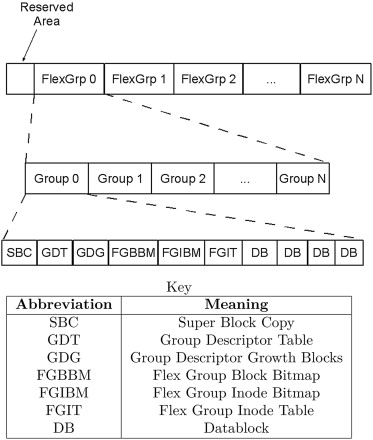
\includegraphics[width=0.36\textwidth]{fig9.jpg}
	\caption{Layout Flexível de Grupos de Blocos}
	\label{fig:9}
\end{figure}

Ao levantar a restrição dos blocos de metadados terem que residir no grupo de blocos ao qual se 
referem, é possível criar um grupo de blocos virtual maior. Isso permite a alocação de blocos de
dados contíguos livres através das fronteiras do grupo. Nas discussões nas listas de desenvolvimento, 
a questão de se as duas opções devem ter diferentes flags de recursos foi abordada. Ficou acordado 
que isso era necessário para manter uma definição clara de \texttt{META\_BG} e \texttt{FLEX\_BG}. 
O recurso \texttt{FLEX\_BG} foi detalhado, pois é selecionado por padrão no arquivo de configuração \texttt{mke2fs}.

\section{Extents (Extensões)}

Outra característica essencial do Ext4 é a adoção de \textit{"extents"} em vez do método de mapeamento 
de blocos previamente utilizado. Os \textit{"extents"} são mais eficientes 
para mapear blocos de dados de arquivos grandes e contíguos, pois sua estrutura inclui o endereço do 
primeiro bloco físico de dados seguido por um comprimento. A Figura \ref{fig:fig10} exibe a estrutura 
do \textit{"extent"} no Ext4, permitindo a sumarização de até 215 blocos com uma única entrada. 
Quando o sistema de arquivos tem um tamanho de bloco de 4 KB, isso mapeia até 128 MB de dados 
com uma única entrada, usando o bit mais alto do campo de comprimento para pré-alocação persistente.

\begin{figure}[H]
    \centering
    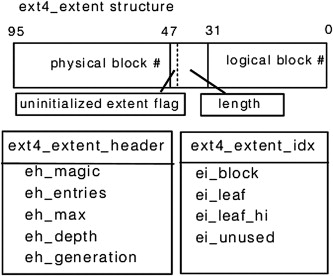
\includegraphics[width=0.5\textwidth]{fig10.jpg}
    \caption{Estrutura do \textit{"extent"} no Ext4 \cite{matur}.}
    \label{fig:fig10}
\end{figure}

De acordo com \cite{matur}, um inode no Ext4 pode conter até quatro \textit{"extents"}. A 
colocação desses \textit{"extents"} no Ext4 é onde anteriormente estavam os ponteiros de bloco no 
Ext3. O formato inclui uma matriz de 60 bytes, com os primeiros 12 bytes contendo um cabeçalho de 
\textit{"extent"}. A estrutura do cabeçalho de \textit{"extent"} é composta pelos campos 
\textit{eh\_magic}, \textit{eh\_entries}, \textit{eh\_max}, \textit{eh\_depth} 
(2 bytes cada) e \textit{eh\_generation} (4 bytes), sendo o número mágico 0xf30A. 
Quando um arquivo é altamente fragmentado, muito grande ou esparsamente distribuído, 
uma árvore de \textit{"extent"} é construída, conforme mostrado na Figura \ref{fig:fig11}.



A estrutura de índice 
de \textit{"extent"} atua como uma estrutura intermediária, apontando para um bloco que 
contém outras estruturas que, por sua vez, apontam para dados. Esta estrutura possui um campo
\textit{ei\_block} (4 bytes) usado para denotar o bloco inicial do arquivo ao qual o índice se 
refere. As árvores de \textit{"extents"} válidas devem aderir a regras específicas, 
como a presença do cabeçalho de \textit{"extent"} em cada nó e a ordenação crescente dos 
campos \textit{ee\_block} em nós folha, além do aumento nos valores \textit{ei\_block} em nós de índice.

É importante observar que essas considerações de \textit{"extents"} proporcionam maior eficiência 
no mapeamento de grandes volumes de dados con@book{carrier2005file,
title={File system forensic analysis},
author={Carrier, Brian},
year={2005},
publisher={Addison-Wesley Professional}
}tíguos, oferecendo benefícios significativos ao 
desempenho e à gestão de espaço em disco no Ext4. Para uma visualização mais detalhada dessas 
estruturas, consulte as Figuras \ref{fig:fig10} e \ref{fig:fig11} em \cite{matur}.

\section{Inodes e Tempo no Ext4}

Como observado por \cite{matur} e \cite{xia}, o Ext3 é limitado à resolução de segundos 
no nível do sistema de arquivos. Isso é abordado no Ext4 modificando e estendendo a estrutura de 
inode. Embora o Ext3 suporte tamanhos diferentes de inode que são potências de dois maiores que 128 
bytes até o tamanho de um bloco de sistema de arquivos, 128 bytes é o tamanho padrão. As estruturas 
mais recentes no Ext4 serão, por padrão, de 256 bytes \cite{matur}. Este espaço permite ao 
Ext4 suportar carimbos de tempo em nanossegundos e números de versão de inode de 64 bits. 
Conforme mostrado na Figura \ref{fig:ext4-inode}, os primeiros 128 bytes permanecem em 
grande parte iguais, enquanto os novos campos são adicionados ao final da estrutura. 
Além disso, um novo campo de carimbo de tempo foi adicionado para documentar o momento 
da criação do arquivo. Cada campo de carimbo de tempo no inode, com exceção do carimbo de tempo de 
exclusão, possui um campo de 32 bits correspondente. Nesse espaço, apenas os 30 bits superiores são 
usados para representação em nanossegundos. Os 2 bits restantes são usados como bits mais significativos 
da segunda parte dos carimbos de tempo, adiando assim o problema de 2038 por 272 anos. 
Essa melhoria na resolução de tempo do ponto de vista do sistema de arquivos pode ser 
útil para pesquisas futuras em forense computacional e segurança. O espaço restante é 
ocupado por atributos estendidos rápidos. Nos primeiros 128 bytes, o número de fragmento 
de 1 byte, o tamanho do fragmento de 1 byte e um campo de preenchimento de 2 bytes foram 
substituídos pelos campos \texttt{i\_blocks\_high} e \texttt{file\_acl\_high}, cada um com 16 bits.

\begin{figure}[H]
  \centering% Definindo cores personalizadas para o código Python    % Para definir cores personalizadas
  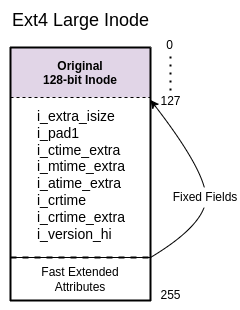
\includegraphics[width=0.34\textwidth]{fig12.png}
  \caption{Ext4 inode. Original apareceu em \cite{matur}.}
  \label{fig:ext4-inode}
\end{figure}

Embora o tamanho padrão dos inodes do Ext4 seja de 256 bytes, sistemas de 
arquivos Ext4 podem ser criados com um tamanho de inode de 128 bytes. Nesse caso, os campos 
\texttt{i\_ctime\_extra}, \texttt{i\_mtime\_extra}, \texttt{i\_atime\_extra}, \texttt{i\_crtime}, 
\texttt{i\_crtime\_extra} e \texttt{i\_version\_hi} não estarão presentes. Para os campos 
relacionados a carimbos de tempo, isso resulta nos benefícios mencionados anteriormente de 
suporte a subsegundos, uma extensão de 2 bits para carimbos de tempo e a perda do carimbo de tempo de criação.

Todas as alterações na estrutura de dados afetaram o \textit{journaling}, pois o JBD (seção \ref{sec:journaling})
foi ramificado para JBD2, que pode suportar o \textit{journaling} de sistemas de arquivos de 32 bits e 64 bits.

\chapter{Desempenho: Benchmarks}

\definecolor{draculapurple}{RGB}{189, 147, 249}
\definecolor{draculagreen}{RGB}{80, 250, 123}
\definecolor{draculayellow}{RGB}{255, 184, 108}
\definecolor{draculacyan}{RGB}{139, 233, 253}
\definecolor{draculared}{RGB}{255, 85, 85}
\definecolor{draculablack}{RGB}{40, 42, 54}
\definecolor{draculawhite}{RGB}{248, 248, 242}
\definecolor{draculagray}{RGB}{68, 71, 90}

\lstdefinestyle{dracula}{
    backgroundcolor=\color{draculablack},   
    commentstyle=\color{draculagreen},
    keywordstyle=\color{draculacyan},
    numberstyle=\tiny\color{draculayellow},
    stringstyle=\color{draculapurple},
    basicstyle=\footnotesize\ttfamily\color{draculawhite},
    breakatwhitespace=false,
    breaklines=true,
    captionpos=b,
    keepspaces=true,
    numbers=left,
    numbersep=5pt,
    showspaces=false,
    showstringspaces=false,
    showtabs=false,
    tabsize=2
}

\lstset{style=dracula}




Nesta seção, apresentamos um conjunto de testes de desempenho realizados em 
sistemas operacionais, utilizando benchmarks que incluem testes de leitura e 
escrita sequencial, bem como testes de leitura e escrita aleatória. Os testes 
foram conduzidos em 12 arquivos, cada um com tamanho de 1GB.

\section{Código de Benchmark}

A seguir, apresentamos o código em Python utilizado para realizar os testes:

\begin{lstlisting}[language=Python, caption=
	{Código de Benchmark. 
	\href{https://github.com/jvictorferreira3301/Sistemas_Operacionais/blob/main/6_ext4/benchmark_ext4.py}{github.com/jvictorferreira3301/SistemasOperacionais
	/blob/main/6\_ext4/benchmark\_ext4.py}}, label=benchmark_code]
	import os
	import time
	import random
	
	def write_sequential(file_path, file_size_mb, block_size_kb):
		with open(file_path, 'wb') as f:
			#7for _ in range(file_size_mb * 1024 // block_size_kb):
			f.write(os.urandom(1024*1024* 1024))
	
	def read_sequential(file_path, block_size_kb):
		with open(file_path, 'rb') as f:
			while f.read(block_size_kb * 1024):
				pass
	
	def write_random(file_path, file_size_mb, block_size_kb):
		with open(file_path, 'wb') as f:
			for _ in range(file_size_mb * 1024 // block_size_kb):
				pos = random.randint(0, file_size_mb * 1024 * 1024 - block_size_kb * 1024)
				f.seek(pos)
				f.write(os.urandom(block_size_kb * 1024))
	
	def read_random(file_path, file_size_mb, block_size_kb):
		with open(file_path, 'rb') as f:
			for _ in range(file_size_mb * 1024 // block_size_kb):
				pos = random.randint(0, file_size_mb * 1024 * 1024 - block_size_kb * 1024)
				f.seek(pos)
				f.read(block_size_kb * 1024)
	
	def run_tests():
		file_size_mb = 1024
		block_size_kb = 4
		num_files = 12
	
		for i in range(1, num_files + 1):
			file_path = f'arquivo{i}.txt'
	
			print(f"Running tests for {file_path}...")
			
			start_time = time.time()
			write_sequential(file_path, file_size_mb, block_size_kb)
			elapsed_time = time.time() - start_time
			print(f"Sequential Write: {elapsed_time:.2f} seconds")
	
			start_time = time.time()
			read_sequential(file_path, block_size_kb)
			elapsed_time = time.time() - start_time
			print(f"Sequential Read: {elapsed_time:.2f} seconds")
	
			start_time = time.time()
			write_random(file_path, file_size_mb, block_size_kb)
			elapsed_time = time.time() - start_time
			print(f"Random Write: {elapsed_time:.2f} seconds")
	
			start_time = time.time()
			read_random(file_path, file_size_mb, block_size_kb)
			elapsed_time = time.time() - start_time
			print(f"Random Read: {elapsed_time:.2f} seconds")
	
	if __name__ == "__main__":
		run_tests()
\end{lstlisting}


O código consiste em funções para realizar testes de leitura e escrita sequencial, 
bem como testes de leitura e escrita aleatória. O desempenho é medido em termos do 
tempo necessário para realizar essas operações. Cada teste é executado em 12 arquivos 
distintos, cada um com um tamanho de 1GB.

\section{Resultados dos Testes}

\subsection{Teste de Leitura Sequencial}

Neste teste, avaliamos o desempenho da leitura sequencial em diferentes arquivos. 
O processo consiste em ler dados de maneira contínua, sem saltos, percorrendo o 
arquivo de início ao fim. A Figura~\ref{fig:sr} apresenta os tempos de leitura 
sequencial para cada arquivo, destacando as variações de desempenho entre eles.

\begin{figure}[H]
    \centering
    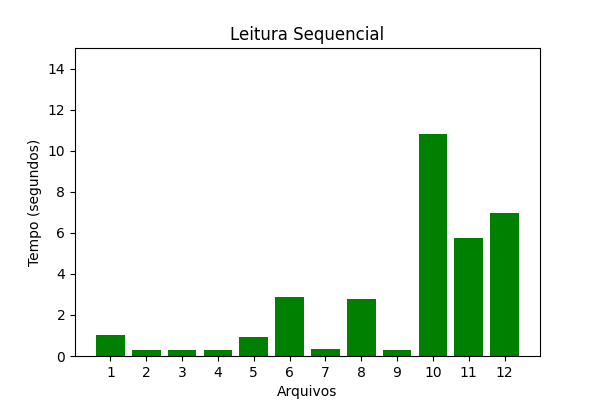
\includegraphics[width=0.7\textwidth]{SeqRead.png}
    \caption{Tempos de Leitura Sequencial para Cada Arquivo.}
    \label{fig:sr}
\end{figure}

% Inclua tabelas ou gráficos com os resultados do teste de leitura sequencial aqui...

\subsection{Teste de Escrita Sequencial}

No teste de escrita sequencial, examinamos como o sistema lida com operações 
de escrita contínua em diferentes arquivos. Isso envolve a gravação de dados 
de maneira consecutiva, sem movimentos aleatórios no arquivo. 
A Figura~\ref{fig:sw} exibe os tempos de escrita sequencial para cada 
arquivo, proporcionando insights sobre a eficiência do sistema em 
operações de escrita ordenada.

\begin{figure}[H]
    \centering
    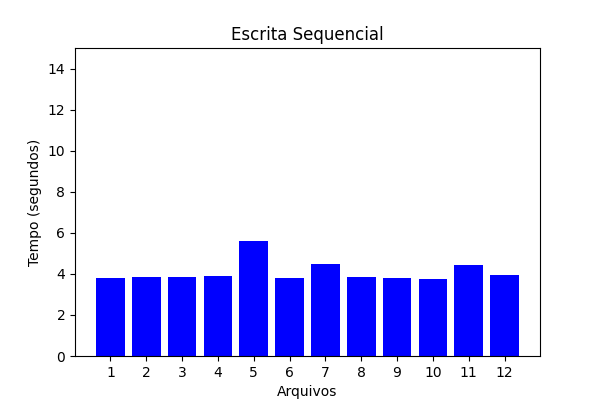
\includegraphics[width=0.7\textwidth]{SeqWrite.png}
    \caption{Tempos de Escrita Sequencial para Cada Arquivo.}
    \label{fig:sw}
\end{figure}

% Inclua tabelas ou gráficos com os resultados do teste de escrita sequencial aqui...

\subsection{Teste de Leitura Aleatória}

No teste de leitura aleatória, avaliamos o desempenho da leitura de dados 
em posições não sequenciais nos arquivos. Isso simula a leitura de dados 
de maneira aleatória, sem seguir uma ordem específica. A Figura~\ref{fig:rr} 
ilustra os tempos de leitura aleatória para cada arquivo, oferecendo uma 
visão do comportamento do sistema diante de operações de leitura não lineares.

\begin{figure}[H]
    \centering
    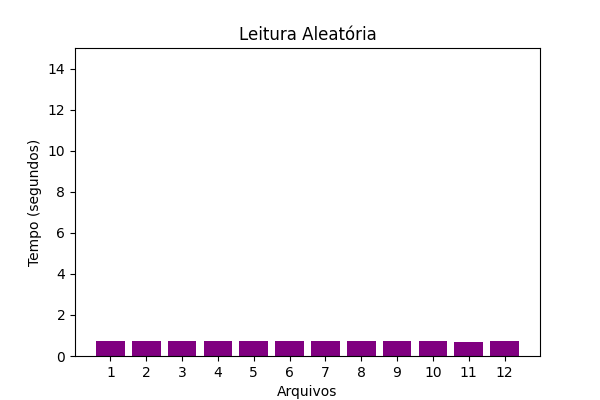
\includegraphics[width=0.7\textwidth]{RandomRead.png}
    \caption{Tempos de Leitura Aleatória para Cada Arquivo.}
    \label{fig:rr}
\end{figure}

% Inclua tabelas ou gráficos com os resultados do teste de leitura aleatória aqui...

\subsection{Teste de Escrita Aleatória}

O teste de escrita aleatória explora como o sistema lida com operações de 
escrita em posições não sequenciais nos arquivos. Isso inclui a gravação 
de dados em locais arbitrários, sem seguir uma ordem específica. 
A Figura~\ref{fig:rw} apresenta os tempos de escrita aleatória para cada arquivo, 
permitindo a análise do desempenho do sistema em cenários de gravação não linear.

\begin{figure}[H]
    \centering
	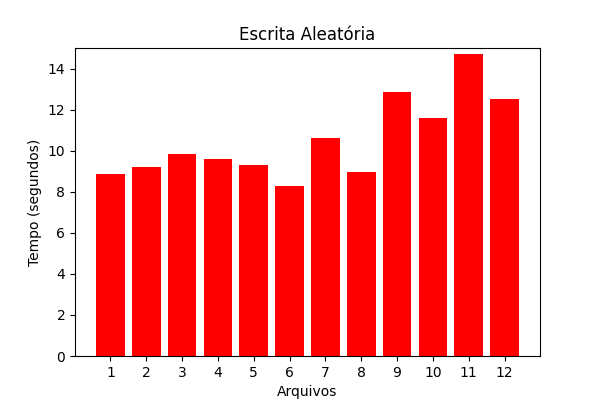
\includegraphics[width=0.7\textwidth]{RandomWrite.png}
    \caption{Tempos de Escrita Aleatória para Cada Arquivo.}
    \label{fig:rw}
\end{figure}

\section{Considerações Importantes para o Benchmark}

Ao analisar os tempos de execução em um benchmark de sistema de arquivos, é crucial levar em 
consideração vários fatores que podem influenciar os resultados. A seguir, destacamos
algumas considerações essenciais:

\subsection{Hardware}

O desempenho do sistema de arquivos é fortemente influenciado pelo hardware 
subjacente. Características como o tipo e a velocidade do disco rígido (HDD), 
o tipo e a configuração do disco de estado sólido (SSD), a quantidade e a 
velocidade da memória RAM, e a capacidade do processador (CPU) podem ter 
impactos significativos nos resultados do benchmark. Em nossa análise foi usado
uma máquina com as características especificadas na tabela \ref{tab:ideapad_specs}


\begin{table}[H]
    \centering
    \caption{Especificações do Hardware usado}
    \begin{tabular}{@{}ll@{}}
        \toprule
        \textbf{Componente} & \textbf{Especificação} \\
        \midrule
        Processador & Intel Core i3-10110U \\
        Memória RAM & 8 GB DDR4 (2x4) 2666 \\
        Armazenamento & SSD NVME 128 GB \\
        Sistema Operacional & Ubuntu 22.04 LTS \\
        \bottomrule
    \end{tabular}
    \label{tab:ideapad_specs}
\end{table}
\subsection{Tipo de Acesso}

Operações de leitura e escrita sequencial geralmente apresentam desempenho superior 
em comparação com operações aleatórias. A otimização do sistema de arquivos 
pode variar de acordo com o tipo específico de acesso.

\begin{figure}[H]
	\centering
	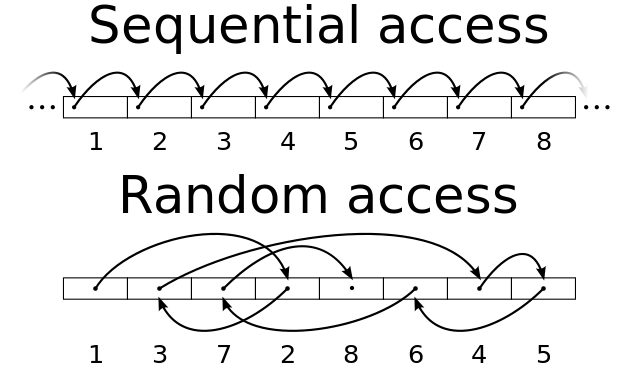
\includegraphics[width=0.5\textwidth]{RandomVsSeq.png}
	\caption{Acessos sequencial e aleatório}
\end{figure}

\subsection{Tamanho dos Arquivos}

O tamanho dos arquivos utilizados nos testes pode influenciar os resultados. 
O comportamento do sistema de arquivos pode ser diferente dependendo do 
tamanho dos arquivos envolvidos.

%\subsection{Cache do Sistema Operacional}

%A presença de cache no sistema operacional pode impactar os tempos de leitura 
%e gravação. Operações subsequentes podem ser aceleradas se os dados estiverem 
%em cache, introduzindo variabilidades nos resultados.


\subsection{Cargas do Sistema}

Outras tarefas em execução no sistema podem impactar o desempenho dos 
testes. Recomenda-se realizar os benchmarks em um sistema relativamente 
inativo, como fizemos em nossa análise, para obter resultados mais consistentes.

\chapter{Conclusão}

Neste trabalho, realizamos benchmarks de desempenho em diferentes cenários 
de acesso a arquivos em um sistema operacional Linux com o sistema de arquivos Ext4, 
utilizando um computador com o hardware descrito na tabela \ref{tab:ideapad_specs}  
como ambiente de teste. Os testes incluíram operações de leitura e escrita 
sequencial, bem como leitura e escrita aleatória, em arquivos de tamanho fixo.

Ao analisar os resultados apresentados no gráfico geral de comparação de desempenho 
(Figura \ref{fig:oneforall}), observamos padrões interessantes. Os tempos de 
escrita sequencial, em geral, mantiveram-se estáveis, enquanto os tempos de 
leitura sequencial e os tempos de leitura e escrita aleatórias variaram 
consideravelmente entre os diferentes arquivos.

\begin{figure}[H]
	\centering
	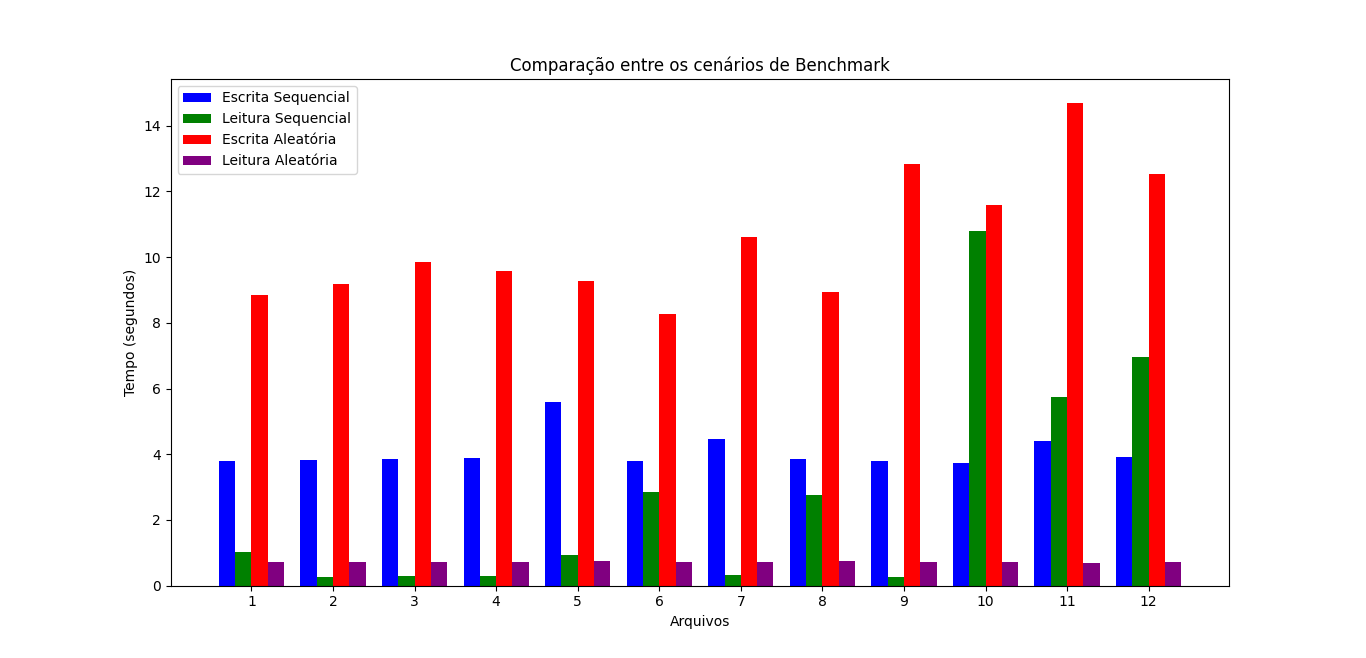
\includegraphics[width=1.0\textwidth]{oneforall_grafico.png}
	\caption{Acessos sequencial e aleatório}
	\label{fig:oneforall}
\end{figure}


Essas variações podem ser atribuídas a uma série de fatores, como a 
alocação de blocos, a presença de cache do sistema operacional, e a 
configuração específica do sistema de arquivos utilizado. É crucial 
considerar esses fatores ao interpretar os resultados.

Em resumo, este estudo fornece insights valiosos sobre o desempenho do 
sistema de arquivos em diferentes cenários. No entanto, para uma compreensão 
mais abrangente, seria necessário realizar análises mais detalhadas, 
considerando diversos parâmetros e cenários adicionais.
\postextual

\bibliography{bibliografia}

\cite{FAIRBANKS2012S118}
\cite{bovet_cesati_2005}
\cite{Tso}
\cite{matur}
\cite{kumar}
\cite{carrier2005file}

\end{document}
